\documentclass[12pt,compress,english,utf8,t]{beamer}
\usepackage[ngerman]{babel}
\usepackage{calc}
\usepackage{ragged2e,wasysym,multicol,mathtools}
\usepackage[protrusion=true,expansion=true]{microtype}
\usepackage{tikz}
\hypersetup{colorlinks=true}

\graphicspath{{images/}}

\title{\large How does artificial intelligence \\ accomplish the feat of
learning?}
\author[Ingo Blechschmidt]{\textcolor{white}{Ingo Blechschmidt \\ \small with
thanks to Tim Baumann and Philipp Wacker}}
\date[2019-12-30]{\vspace*{-5em}\ \\\textcolor{white}{\scriptsize University of
Augsburg \\ 36th Chaos Communication Congress \\}}

\useinnertheme[shadow=true]{rounded}
\useoutertheme{split}
\usecolortheme{orchid}
\usecolortheme{whale}
\setbeamerfont{block title}{size={}}

\useinnertheme{rectangles}

\usecolortheme{seahorse}
\definecolor{mypurple}{RGB}{150,0,255}
\setbeamercolor{structure}{fg=mypurple}
\definecolor{myred}{RGB}{150,0,0}
\setbeamercolor*{title}{bg=myred,fg=white}
\setbeamercolor*{titlelike}{bg=myred,fg=white}

\usefonttheme{serif}
\usepackage[T1]{fontenc}
\usepackage{libertine}

\renewcommand{\_}{\mathpunct{.}\,}
\newcommand{\BB}{\mathbb{B}}
\newcommand{\M}{\mathcal{M}}
\newcommand{\R}{\mathrm{R}}
\newcommand{\NN}{\mathbb{N}}
\newcommand{\RR}{\mathbb{R}}

\setbeamertemplate{navigation symbols}{}

\setbeamertemplate{title page}[default][colsep=-1bp,rounded=false,shadow=false]
\setbeamertemplate{frametitle}[default][colsep=-2bp,rounded=false,shadow=false,center]

\newcommand{\hil}[1]{{\usebeamercolor[fg]{item}{\textbf{#1}}}}
\setbeamertemplate{frametitle}{%
  \vskip1em%
  \leavevmode%
  \begin{beamercolorbox}[dp=1ex,center]{}%
      \usebeamercolor[fg]{item}{\textbf{\textsf{\Large \insertframetitle}}}
  \end{beamercolorbox}%
}

\setbeamertemplate{footline}{%
  \leavevmode%
  \hfill%
  \begin{beamercolorbox}[ht=2.25ex,dp=1ex,right]{}%
    \usebeamerfont{date in head/foot}
    \insertframenumber\,/\,\inserttotalframenumber\hspace*{1ex}
  \end{beamercolorbox}%
  \vskip0pt%
}

\newcommand{\backupstart}{
  \newcounter{framenumberpreappendix}
  \setcounter{framenumberpreappendix}{\value{framenumber}}
}
\newcommand{\backupend}{
  \addtocounter{framenumberpreappendix}{-\value{framenumber}}
  \addtocounter{framenumber}{\value{framenumberpreappendix}}
}

\setbeameroption{show notes}
\setbeamertemplate{note page}[plain]

\newcommand{\imgslide}[3]{{\usebackgroundtemplate{\parbox[c][\paperheight][c]{\paperwidth}{\centering\includegraphics[width=\paperwidth]{#1}}}\begin{frame}[plain,b]\tiny Quelle: \href{#2}{#3}\par\end{frame}}}

\newcommand{\portrait}[4]{\begin{column}{#3\textwidth}\centering\includegraphics[height=#4\textheight]{#1}\\{\scriptsize #2\par}\end{column}}

\begin{document}

% https://static2.gamespot.com/uploads/original/1557/15576725/2944861-hogwarts.jpg
{\usebackgroundtemplate{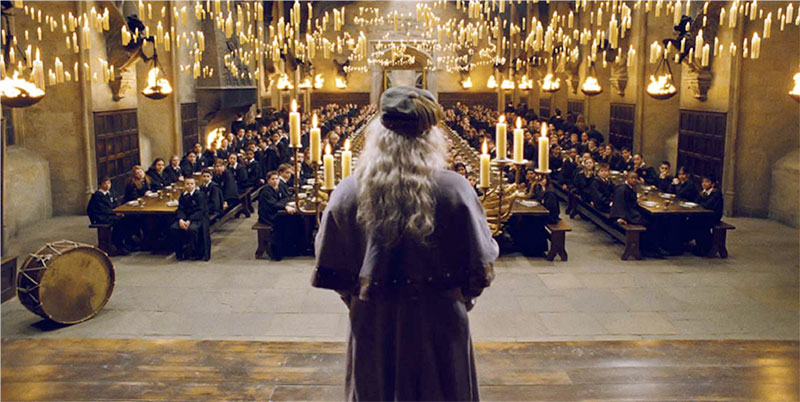
\includegraphics[height=\paperheight]{hogwarts}}
\frame{\vspace*{9em}\titlepage}}
\frame{\tableofcontents}

% Einführungsvideos
% * https://www.youtube.com/watch?v=MzJ0CytAsec
%   Windows Vista Speech Recognition Tested - Perl Scripting
% * https://www.youtube.com/watch?v=M1ONXea0mXg
%   Hound Internal Demo

\section[Successes]{Successes of AI}

\begin{frame}
  \centering
  \bigskip\bigskip

  \Huge \hil{Part I}

  \bigskip
  \Large\textbf{Recent successes of \\ artificial intelligence}
  \par

  \vfill
  \vfill
  \vfill
  \begin{columns}
    % http://nerdist.com/wp-content/uploads/2016/03/DeepMind-Sedol-Go-Match-Feature-Image-03082016.jpg
    \portrait{wavenet}{\href{https://deepmind.com/blog/wavenet-generative-model-raw-audio/}{Speech synthesis}}{0.17}{0.25}
    \portrait{deepmind-match}{\href{https://de.wikipedia.org/wiki/AlphaGo}{AlphaGo}}{0.25}{0.25}
    \portrait{neural-style}{\href{https://github.com/jcjohnson/neural-style}{Style transfer}}{0.25}{0.25}
    \portrait{magenta-jam-session}{\href{https://magenta.tensorflow.org/blog/2016/12/16/nips-demo/}{Jam with Magenta}}{0.25}{0.25}
  \end{columns}
\end{frame}

% Für Wavenet abspielen: resources/speaker-*.wav
% Für Stiltransfer: resources/jcjohnson*.html
% Für die Supervergrößerung: resources/neural-enhance.gif


\section[How?]{How artificial neural networks work}

{\usebackgroundtemplate{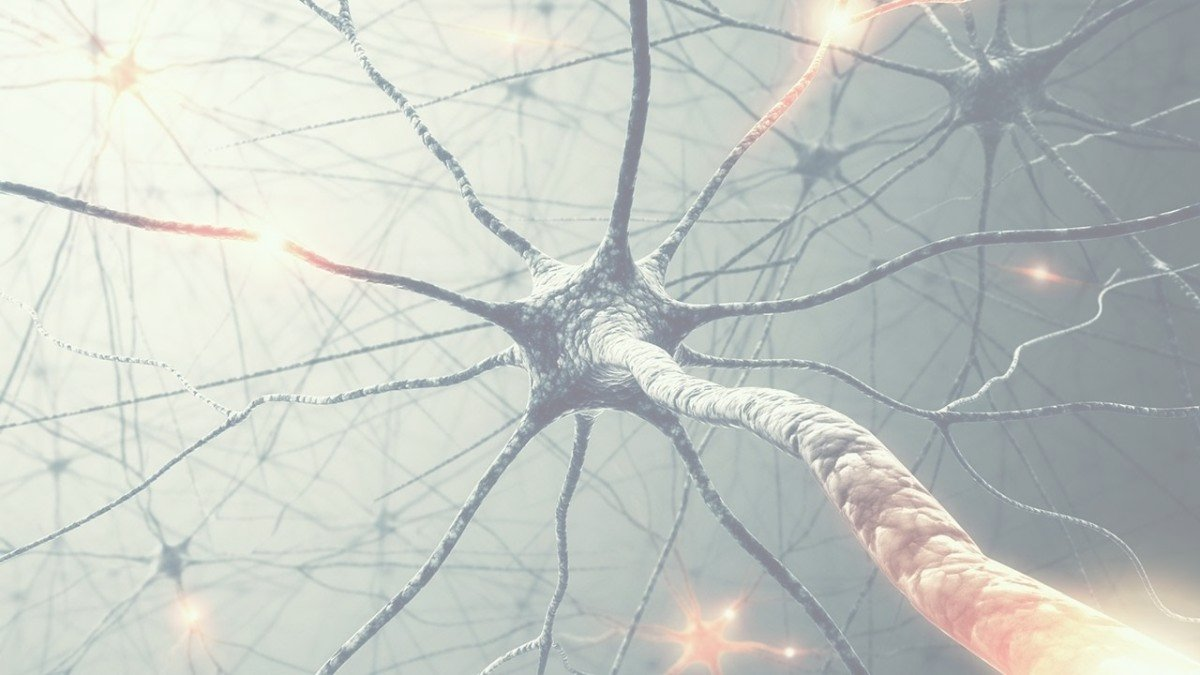
\includegraphics[height=\paperheight]{neuron-art}}
\begin{frame}
  \centering
  \bigskip\bigskip

  \Huge \hil{Part II}

  \bigskip
  \Large\textbf{How artificial neural networks work}
  \par

  \vfill\small
  \begin{enumerate}
    \item Architecture of a simple net
    \item Valuation by a cost function
    \item Error minimization using gradient descent
  \end{enumerate}
\end{frame}}


\begin{frame}{The MNIST database}
  \centering
  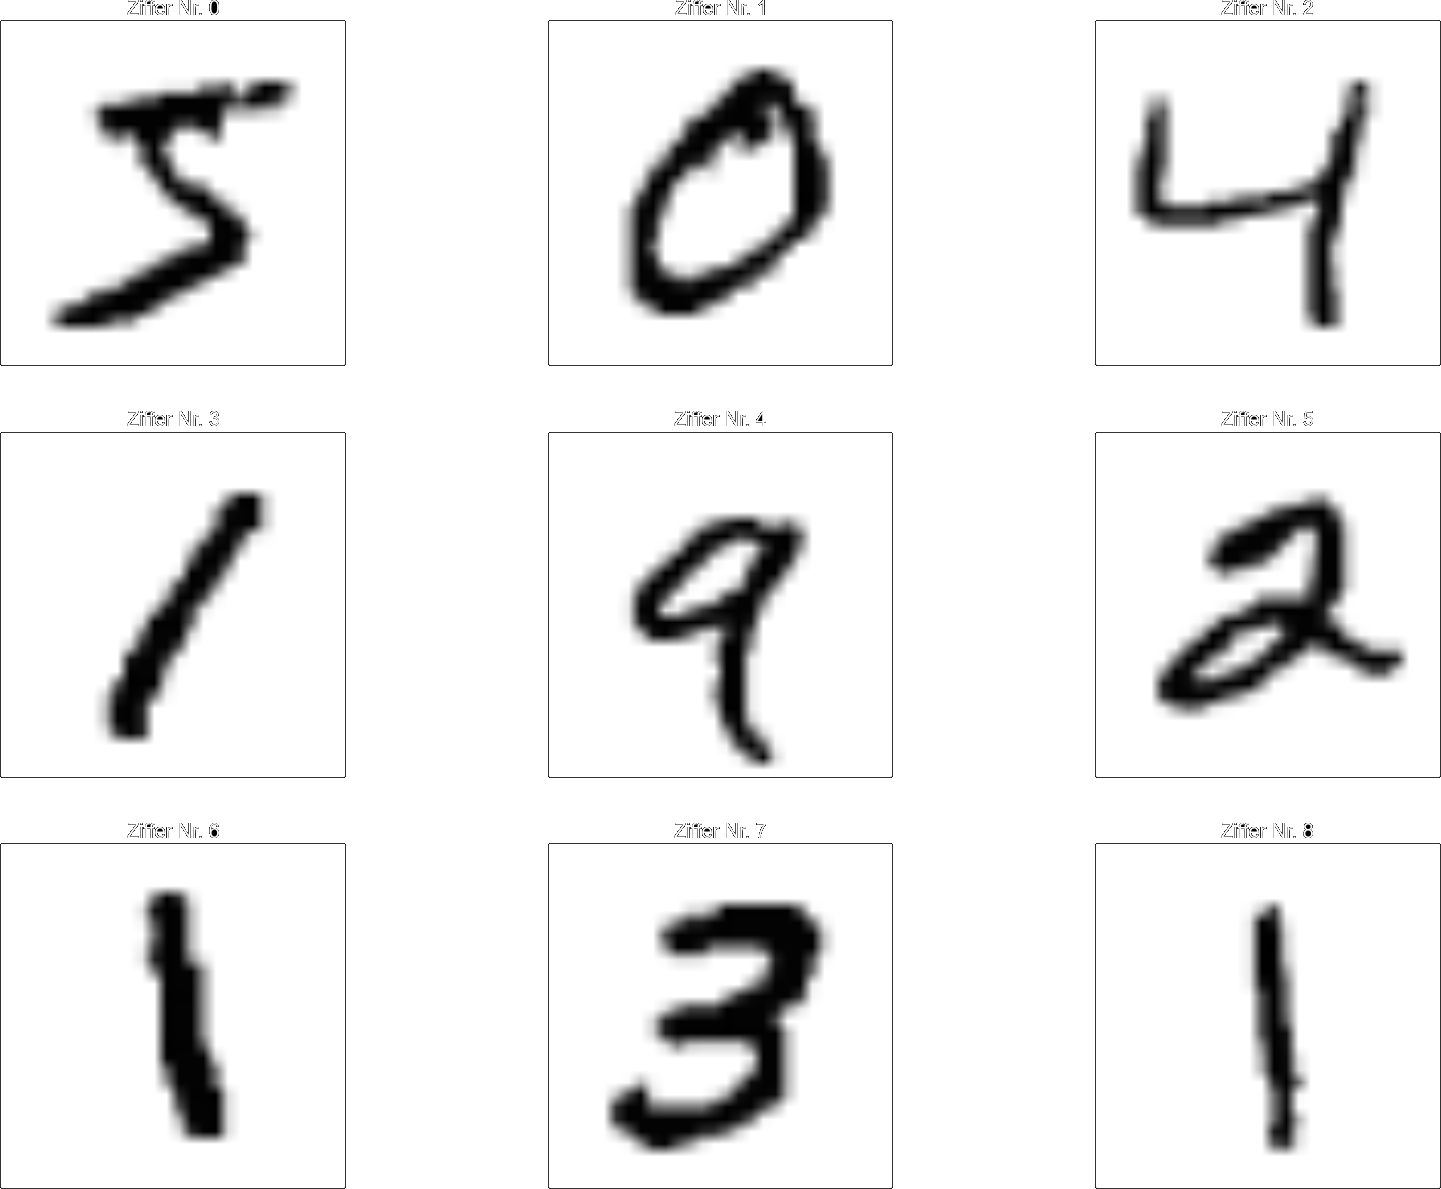
\includegraphics[width=0.7\textwidth]{mnist-ziffern}
  \bigskip

  70\,000 images consisting of $28 \times 28$ pixels
  \par
\end{frame}


\subsection{Architecture}

% Vorlage von Kjell Magne Fauske, http://www.texample.net/tikz/examples/neural-network/
\begin{frame}{Architecture of a simple net}
  \def\layersep{2cm}
  \begin{tikzpicture}[shorten >=1pt,->,draw=black!50, node distance=\layersep]
    \tikzstyle{every pin edge}=[<-,shorten <=1pt]
    \tikzstyle{every node}=[font={\small}]
    \tikzstyle{neuron}=[circle,fill=black!25,minimum size=17pt,inner sep=0pt]
    \tikzstyle{input neuron}=[neuron, fill=green!80];
    \tikzstyle{output neuron}=[neuron, fill=red!50];
    \tikzstyle{hidden neuron}=[neuron, fill=blue!50];
    \tikzstyle{annot} = [text width=4em, text centered]

    \node[input neuron, pin=left:input 1] (I-1) at (0,-1.2*1) {\only<3->{$0.1$}};
    \node[input neuron, pin=left:input 2] (I-2) at (0,-1.2*2) {\only<3->{$0.7$}};
    \node[input neuron, pin=left:input 3] (I-3) at (0,-1.2*3) {\only<3->{$0.2$}};
    \node[input neuron, pin=left:input 4] (I-4) at (0,-1.2*4) {\only<3->{$0.4$}};

    \foreach \name / \y in {1,...,5}
      \path[yshift=0.5cm]
        node[hidden neuron] (H-1-\name) at (\layersep,-1.2*\y cm) {};
    \foreach \name / \y in {1,...,5}
      \path[yshift=0.5cm]
        node[hidden neuron] (H-2-\name) at (2*\layersep,-1.2*\y cm) {};

    \only<5->{
      \node at (H-1-2) {$y$};
    }

    \node[output neuron,pin={[pin edge={->}]right:output 1}, right of=H-2-2] (O-1) {};
    \node[output neuron,pin={[pin edge={->}]right:output 2}, right of=H-2-4] (O-2) {};

    \only<1>{
      \foreach \source in {1,...,4}
        \foreach \dest in {1,...,5}
          \path (I-\source) edge (H-1-\dest);
    }
    \only<2->{
      \foreach \source in {1,...,4}
        \foreach \dest in {2}
          \path (I-\source) edge (H-1-\dest);
    }
    \only<4->{
      \path (I-1) -- (H-1-2) node[midway] {3};
      \path (I-2) -- (H-1-2) node[midway] {4};
      \path (I-3) -- (H-1-2) node[midway] {1};
      \path (I-4) -- (H-1-2) node[midway] {5};
    }
    \only<1>{
      \foreach \source in {1,...,5}
        \foreach \dest in {1,...,5}
          \path (H-1-\source) edge (H-2-\dest);
    }
    \only<2->{
      \foreach \source in {2}
        \foreach \dest in {1,...,5}
          \path (H-1-\source) edge (H-2-\dest);
    }

    \foreach \source in {1,...,5}
      \path (H-2-\source) edge (O-1);
    \foreach \source in {1,...,5}
      \path (H-2-\source) edge (O-2);

    \node[annot,above of=H-1-1, node distance=1cm] (hl1) {hidden layer};
    \node[annot,above of=H-2-1, node distance=1cm] (hl2) {hidden layer};
    \node[annot,left of=hl1] {input layer};
    \node[annot,right of=hl2] {output layer};

    \only<5->{
      \node[below of=O-2] (y) {\scriptsize $y = \sigma(0.1\cdot3 + 0.7\cdot4 + 0.2\cdot1 + 0.4\cdot5 + b)$};
      \draw[<-, in=120] (H-1-2.east)++(-0.1cm,0cm) to (y.west);
    }

    \only<5->{
      \node at (7.5,-1.2*4.5) {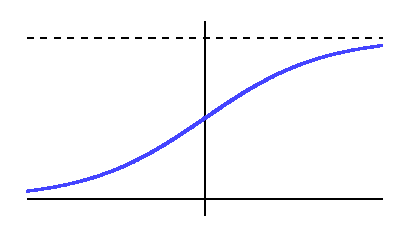
\includegraphics[scale=0.4]{sigmoid}};
    }
  \end{tikzpicture}
\end{frame}


\subsection{Learning by gradient descent}

\begin{frame}{The curious importance of minimization}
  \centering
  \only<1>{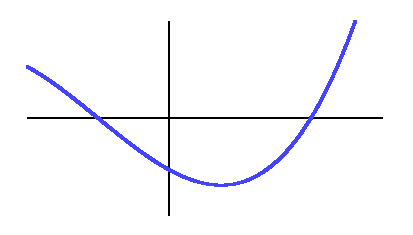
\includegraphics[width=0.8\textwidth]{cubic-polynomial} \par one unknown: $x$}
  \only<2>{\vspace*{-1em}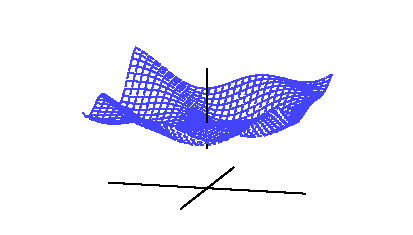
\includegraphics[width=1.0\textwidth]{3d-plot} \par two unknowns: $x$, $y$}
  \only<3>{
    \begin{columns}
      \portrait{leibniz}{\href{https://de.wikipedia.org/wiki/Gottfried_Wilhelm_Leibniz}{Leibniz (* 1646, † 1716)}}{0.3}{0.5}
      \portrait{newton}{\href{https://de.wikipedia.org/wiki/Isaac_Newton}{Newton (* 1643, † 1727)}}{0.3}{0.5}
    \end{columns}
    \bigskip

    arbitrarily many unknowns
    \bigskip
  }
  \par
\end{frame}

\begin{frame}{The feat of learning}
  \begin{enumerate}
    \item Calculate for all of the~60\,000 training cases the activations of
    the ten output neurons.
    \item Sum for all of the resulting 600\,000 activations the individual
    \hil{quadratic errors} to obtain the \hil{total costs}:
    \small
    \begin{align*}
      &\mathop{\phantom{+}} \underbrace{(0.1 - 0)^2 + (0.7 - \hil{1})^2 + (0.1 - 0)^2 + \cdots + (0.2 - 0)^2}_{\text{first test case (should be a one)}} \\[0.3em]
      &+ \underbrace{(0.3 - \hil{1})^2 + (0.2 - 0)^2 + (0.2 - 0)^2 + \cdots + (0.1 - 0)^2}_{\text{second test case (should be a zero)}} \\[0.3em]
      &+ \cdots
    \end{align*}
    \normalsize
    \item Change the weights and biases slightly in the direction of the
    \hil{steepest descent} to very slightly improve performance.
    \item Go to step{\setcounter{enumi}{1}\usebeamercolor[fg]{enumerate item}\usebeamertemplate{enumerate item}}.
  \end{enumerate}
\end{frame}

\note{\justifying\scriptsize
  Im MNIST-Beispiel legen wir von den 70\,000 Einträgen 10\,000
  beiseite; diese verwenden wir später zur Validierung. Den Lernvorgang
  beginnen wir mit einer rein zufälligen Wahl von Gewichten und Biases.
  \begin{enumerate}\justifying
    \item Wir berechnen für jede der 60\,000 Trainingsfälle die
    Aktivierungen der zehn Ausgabeneuronen. So erhalten wir insgesamt 600\,000
    Zahlen zwischen~$0$ und~$1$. Für jedes dieser Ergebnisse wissen wir, welchen
    Wert wir uns eigentlich wünschen (jeweils~$0$ oder~$1$ -- etwa soll
    Ausgabeneuron Nr.~5 bei Eingabe einer handschriftlichen Sieben idealerweise
    überhaupt nicht feuern).
    \item Für jede dieser 600\,000 Ergebnisse berechnen
    wir den \emph{quadratischen Fehler} \[ (\text{tatsächliches Ergebnis} -
    \text{Wunschergebnis})^2 \] und summieren all diese Quadrate auf.
    (Interessiert dich, wieso man hier quadriert? Schreibe eine Mail an
    \href{mailto:iblech@speicherleck.de}{iblech@speicherleck.de}.)
    \item Je größer diese Summe ist, desto schlechter funktioniert das Netzwerk
    auf den Trainingsdaten. Wir möchten daher die Summe \emph{minimieren}. Die
    Summe hängt von den Gewichten der künstlichen Synapsen und den Biases der
    Neuronen ab; diese Abhängigkeit heißt auch \emph{Kostenfunktion}.
    \item Durch Bestimmung des \emph{Gradienten} wissen wir, wie wir die
    Gewichte und Biases ändern müssen, um
    eine kleine Reduktion der Kostenfunktion zu erreichen. So erhalten wir neue
    Gewichte und Biases. Anschließend beginnen wir wieder bei Schritt~1. Auf
    diese Weise folgen wir zu jedem Zeitpunkt der Richtung des steilsten
    Abstiegs im hochdimensionalen Kostengebirge.
  \end{enumerate}
  Sobald wir mit der Leistung des Netzes auf den
  Validierungsdatensätzen zufrieden sind, beenden wir das Training.  Das
  \emph{Wunder der Generalisierung} setzt ein: Das Netz klassifiziert auch
  neu geschriebene Ziffern, die nicht Teil des Trainingdatensatzes waren, sehr
  häufig richtig.\par\bigskip
}


\subsection[Hidden layer]{A look into the hidden layer}

\begin{frame}{A look into the hidden layer}
  \centering
  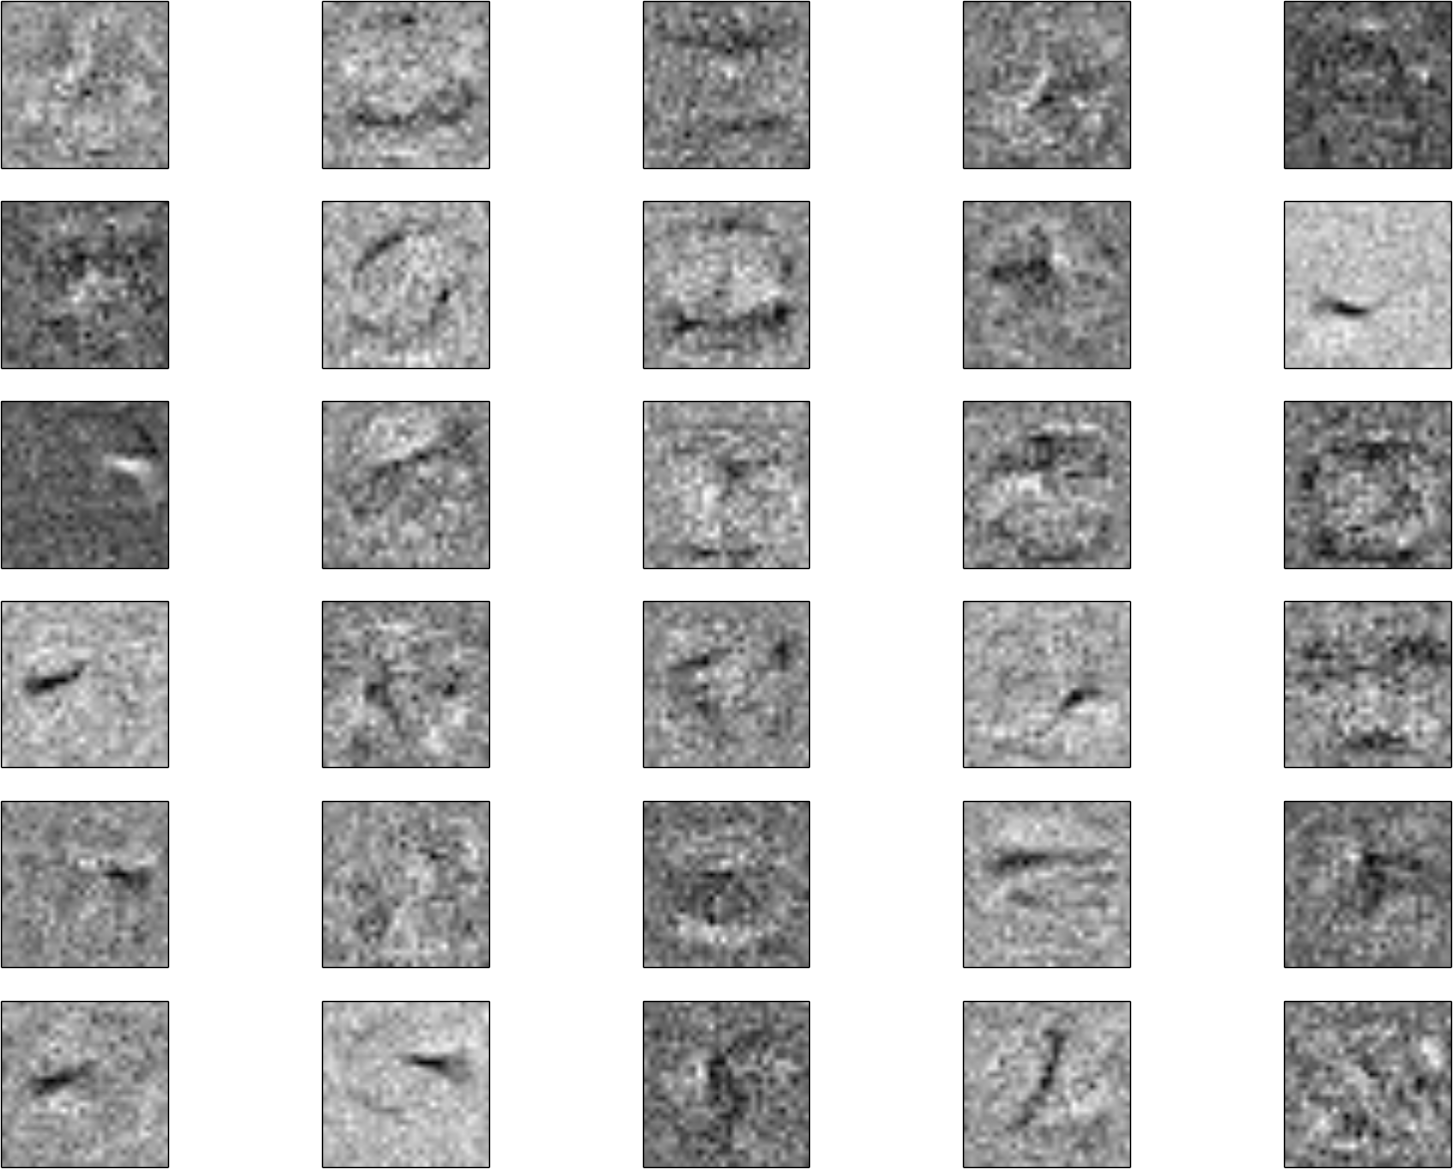
\includegraphics[width=0.8\textwidth]{blick-in-die-zwischenschicht}
  \par
\end{frame}

\note{\justifying
  Hier wurde ein einfaches Netz zur Ziffernerkennung bestehend aus nur einer
  einzigen verborgenen Schicht mit~30 Neuronen trainiert. Die Grafik zeigt die
  Gewichte der Synapsen zwischen den $28 \times 28$ Eingabeneuronen und diesen
  30~Neuronen. Das Netz hat eine Erkennungsrate von~95\,\%.
  \bigskip

  Verwendet man~100 Neuronen, so erreicht man~97\,\%; das ist fast eine
  Halbierung der Fehlerrate.
  \bigskip

  Demo zum Selbstprobieren:
  \begin{itemize}
    \item
    \href{https://github.com/iblech/mathematik-der-vorhersagen/blob/master/neuronale-netze/ziffern/demo.py}{Python-Code
    zur Erkennung}
    \item
    \href{https://github.com/iblech/mathematik-der-vorhersagen/blob/master/neuronale-netze/ziffern/ziffernerkennung-basic.py}{Python-Code
    zum Training}
  \end{itemize}
}


\section[Why not sooner?]{Why not sooner?}

{\usebackgroundtemplate{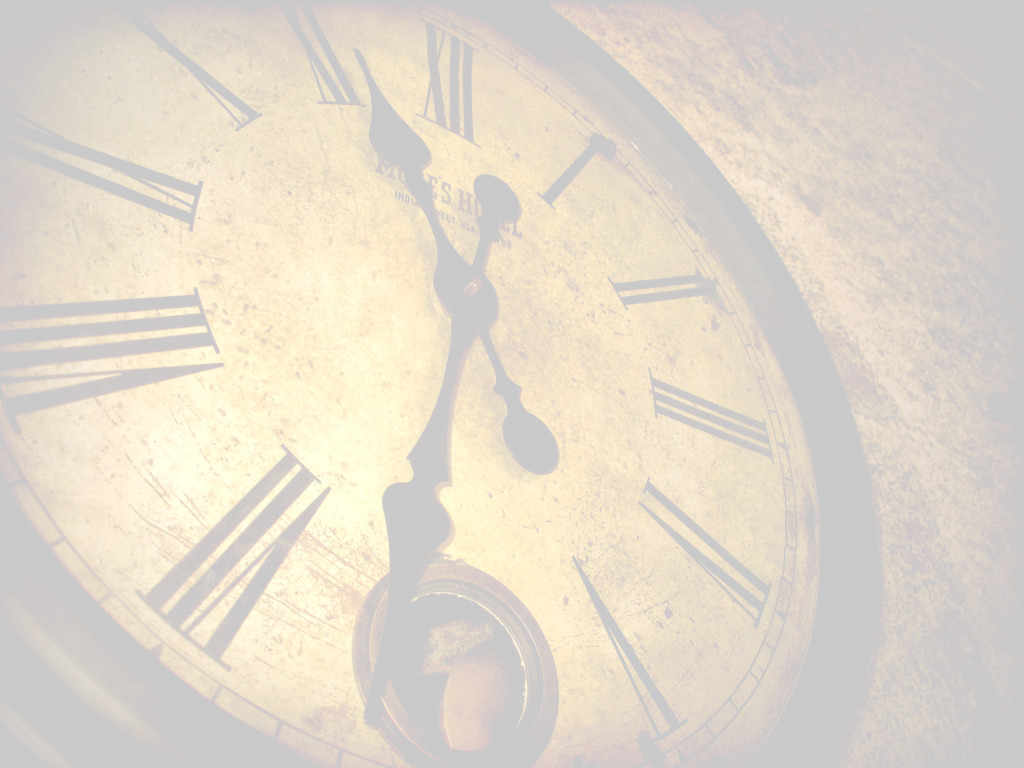
\includegraphics[height=\paperheight]{zeit}}
\begin{frame}
  \centering
  \bigskip\bigskip

  \Huge \hil{Part III}

  \bigskip
  \Large\textbf{Why not sooner?}
  \par

  \vfill\small
  \begin{enumerate}
    \item More computational power
    \pause
    \item Availability of large data sets for training
    \pause
    \item Mathematical breakthrough: Convolutional Neural Networks
  \end{enumerate}
\end{frame}}

% XXX: Bild von CNN einfügen


\section[Onwards]{Challenges for the future}

% http://www.bundesheer.at/archiv/a2005/edelweiss_raid/galerie/vollbild/weitergehts2.jpg
{\usebackgroundtemplate{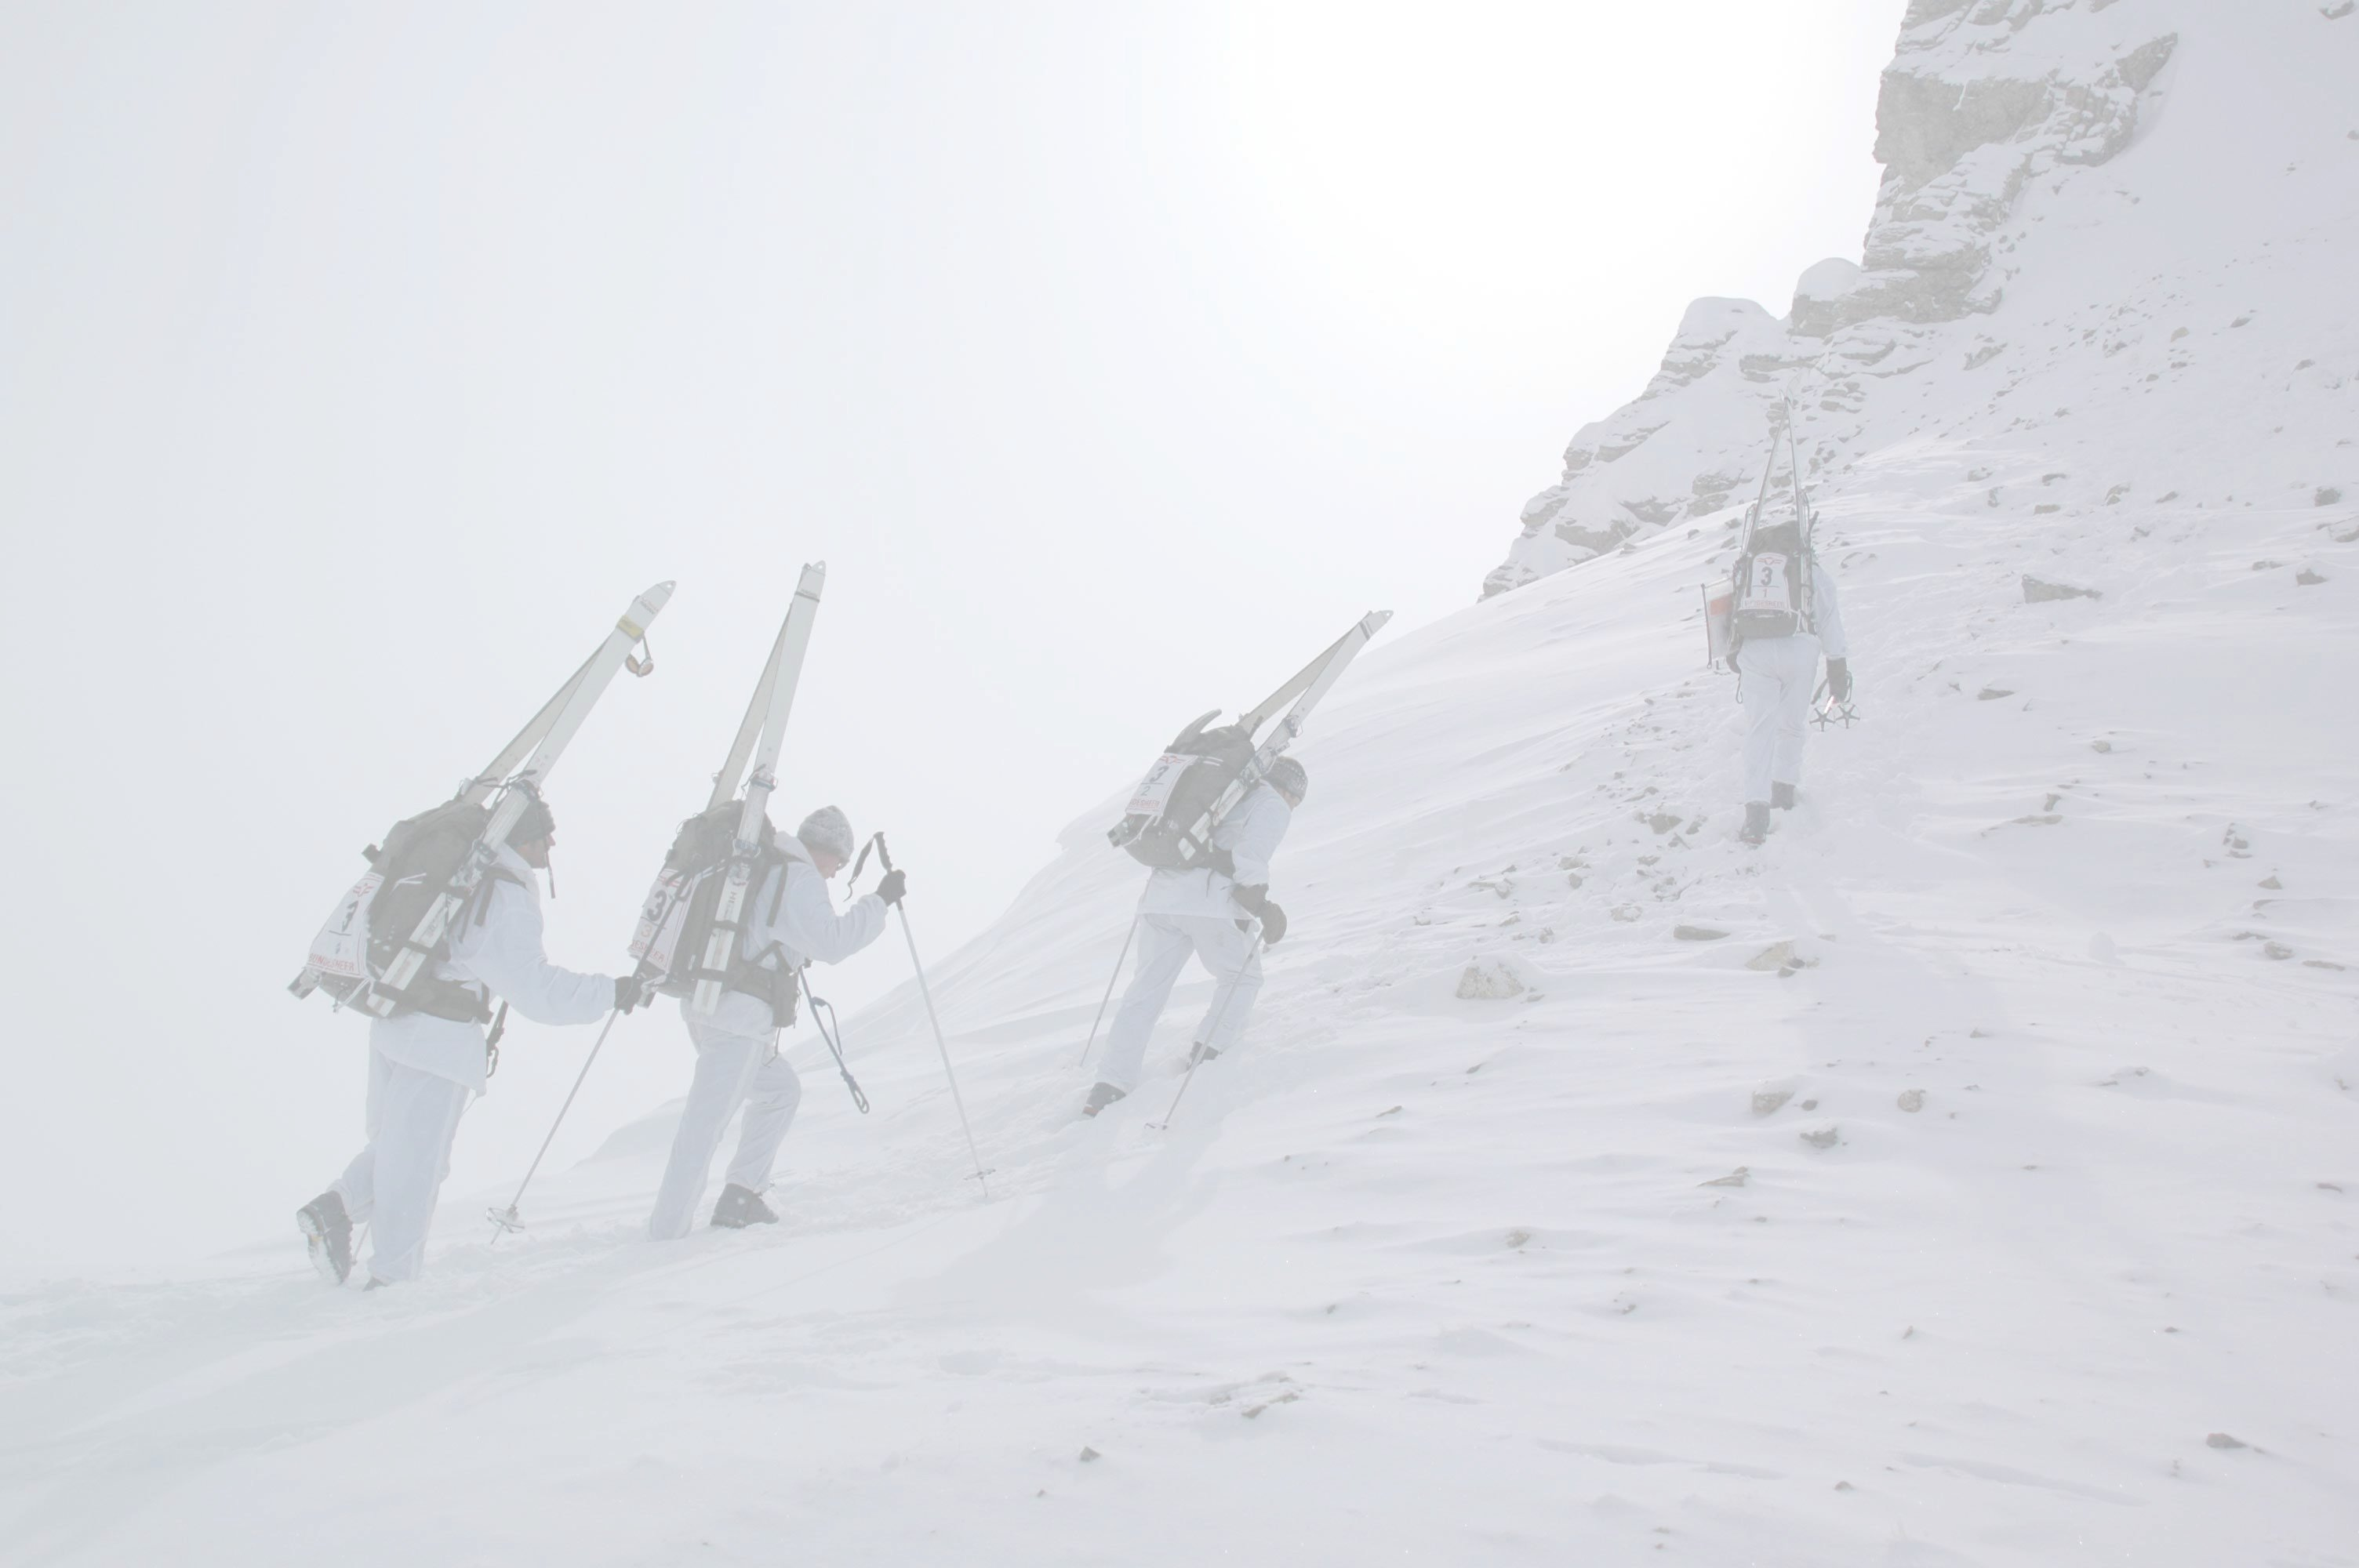
\includegraphics[height=\paperheight]{herausforderung}}
\begin{frame}
  \centering
  \bigskip\bigskip

  \Huge \hil{Part IV}

  \bigskip
  \Large\textbf{Challenges for the future}
  \par

  \vfill\small
  \begin{itemize}
    \item Extend neural nets to further tasks
    \item Understand the inner workings of a trained net
    \item Develop resistence against \href{https://blog.openai.com/adversarial-example-research/}{adversarial examples}
    \item Solve ethical challenges with self-driving cars
    \item Answer existential questions regarding strong AI
  \end{itemize}
\end{frame}}

\note{\justifying
  \emph{Wie} ein künstliches neuronales Netzwerk funktioniert, ist -- anders
  als bei herkömmlichem Programmcode -- nicht klar.
  (Wie beim Menschen auch.) Dazu wird momentan aktiv geforscht. Zwei
  Einstiegspunkte zu solchen Untersuchungen sind:

  \begin{itemize}
    \item \href{https://research.googleblog.com/2015/06/inceptionism-going-deeper-into-neural.html}{Inceptionism:
    Going Deeper into Neural Networks} von Alexander Mordvintsev, Christopher
    Olah und Mike Tyka
    \item \href{http://www.matthewzeiler.com/pubs/arxive2013/eccv2014.pdf}{Visualizing
    and Understanding Convolutional Networks} von Matthew Zeiler und Rob Fergus
  \end{itemize}
}


\section{Recommendations}

{\usebackgroundtemplate{
\includegraphics[height=\paperheight]{westworld}}
\begin{frame}
  \centering
  \bigskip\bigskip

  \Huge \hil{Part V}

  \bigskip
  \Large\textbf{Recommendations}
  \par

  \vfill\small
  \begin{itemize}
    \item HBO series \emph{Westworld} about androids who pass the Turing test
    and develop consciousness
    \item \href{https://www.youtube.com/watch?v=lKQ0yaEJjok}{Talks by
    Joscha Bach on previous congresses}
    \item \href{https://karpathy.github.io/2015/05/21/rnn-effectiveness/}{The
    Unreasonable Effectiveness of Recurrent Neural Networks} by Andrej
    Karpathy
    \item TensorFlow -- AI development without prerequisites in maths
    \item \href{http://neuralnetworksanddeeplearning.com/}{Neural Networks and Deep Learning by Michael Nielsen}
  \end{itemize}
\end{frame}}

\end{document}

% TODO for tomorrow:
% * Find AlphaGo image
% * Preload style transfer website
% * 
